%!TEX TS-program = xelatex
\documentclass[]{friggeri-cv}
\usepackage{afterpage}
\usepackage{hyperref}
\usepackage{color}
\usepackage[utf8]{inputenc} 
\usepackage{xcolor}
%\usepackage{xhfill}
\usepackage{listings}
\definecolor{mygray}{gray}{0.75}
%trials
\usepackage{{ccicons}}
 \usepackage{ifsym}
 \newcommand*{\pin}{%
  
\includegraphics[height=\heightof{M}]{pin}%
}
\newcommand*{\LinkedinLogo}{%
  
\includegraphics[height=\heightof{M}]{LinkedInLogo}%
}
\newcommand*{\SkypeLogo}{%
  
\includegraphics[height=\heightof{M}]{SkypeLogo}%
}
\newcommand*{\GithubLogo}{%
  
\includegraphics[height=\heightof{M}]{GithubLogo}%
}
%\usepackage[default,otf,light]{sourcesanspro}
\usepackage{marvosym}
\hypersetup{
    pdftitle={},
    pdfauthor={},
    pdfsubject={},
    pdfkeywords={},
    colorlinks=false,       % no lik border color
   allbordercolors=white    % white border color for all
}
\addbibresource{bibliography.bib}
\RequirePackage{xcolor}
\definecolor{pblue}{RGB}{0,109,176}

\begin{document}
\header{Sergi}{ Salgueiro Genís}
      {Electronic Engineer}
      
% Fake text to add separator      
%\fcolorbox{white}{gray}{\parbox{\dimexpr\textwidth-2\fboxsep-2\fboxrule}{%
%.....
%}}

%\ccAttribution
% In the aside, each new line forces a line break
\begin{aside}
\tikz[x=1.8cm,y=0cm]{\draw[line width=1mm,gray](-1,1)--(1,-1);}
\section{\textcolor{gray}{\LARGE Info}}
\tikz[x=1.8cm,y=0cm]{\draw[line width=1mm,gray](-1,1)--(1,-1);}
   %\section{{\Gentsroom\hskip 3pt Personal Info}}
   %26 Years old
   %Male
   % \section{{\Mundus\hskip 3pt Personal Website}}
   %\href{http://dbizopoulos.com}{http://dbizopoulos.com}
   %\section{{\pin\hskip 3pt Address}}
    %Kagsåkollegiet 153-16 
    %2860, Søborg, Denmark
  \section{\Telefon\hskip 3pt   Telephone}
  	+34 673550046
%    \section{\SkypeLogo\hskip 3pt  Skype}
%    Username: mpizosdim
%    ~
  \section{\Letter\hskip 3pt   Mail}
    \href{mailto:sergisalgueiro@gmail.com}{sergisalgueiro@\\gmail.com}
  \section{\LinkedinLogo\hskip 3pt  LinkedIn}
    \href{https://dk.linkedin.com/in/sergi-salgueiro-genis}{Sergi Salgueiro Gen\'{i}s}  
  \section{\GithubLogo\hskip 3pt Github}
    \href{https://github.com/sergisalgueiro}{github.com/sergisalgueiro}
%\line(1,0){100}
\tikz[x=1.8cm,y=0cm]{\draw[line width=1mm,gray](-1,1)--(1,-1);}
\section{\textcolor{gray}{\LARGE Skills}}
\tikz[x=1.8cm,y=0cm]{\draw[line width=1mm,gray](-1,1)--(1,-1);}
  \section{Software}
    \textbf{MATLAB / Simulink}\\%
\includegraphics[scale=0.17]{img/4starNew}
    \textbf{C / C++}\\%
\includegraphics[scale=0.17]{img/3starNew}
    %\textbf{R}
\includegraphics[scale=0.17]{img/3starNew}
    \textbf{LaTeX}\\%
\includegraphics[scale=0.17]{img/4starNew}
    \textbf{Python}\\%
\includegraphics[scale=0.17]{img/2starNew}    
    \textbf{TCL/Tk}\\%
\includegraphics[scale=0.17]{img/4starNew}
    \textbf{LabVIEW}\\%
\includegraphics[scale=0.17]{img/1starNew}
    \textbf{M.Office}\\%
\includegraphics[scale=0.17]{img/3starNew}
  \section{Personal Skills}
    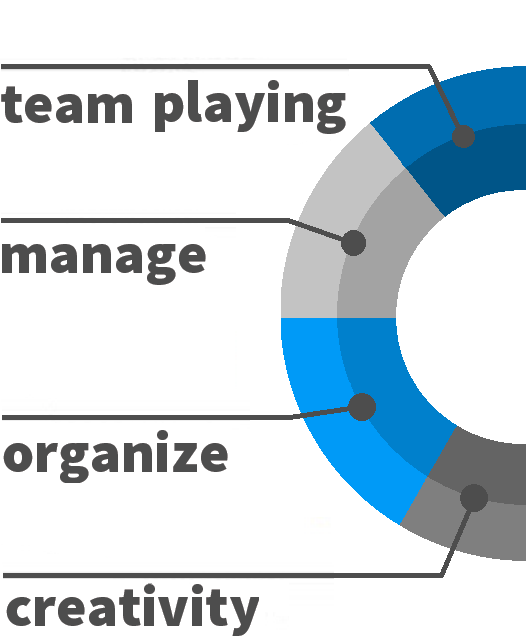
\includegraphics[scale=0.6]{img/PersonalSkillsPhoto.png}
  \section{Languages}
    \textbf{Catalan}
\includegraphics[scale=0.17]{img/5starNew.png}
    \textbf{Spanish}
\includegraphics[scale=0.17]{img/5starNew.png}
    \textbf{English}
\includegraphics[scale=0.17]{img/4starNew.png}
    \textbf{French}
\includegraphics[scale=0.17]{img/4starNew.png}
    %\textbf{Italian}
\includegraphics[scale=0.17]{img/2starNew.png}
    %\textbf{Danish}
\includegraphics[scale=0.17]{img/1starNew.png}
%    \section{Work/Play Balance}
%   
\includegraphics[scale=0.62]{img/personalTrial.png}
%    ~
\end{aside}

\section{Education}
\begin{entrylist}
  \entry
    {2014 - 2016}
    {Master's Degree in Electric Engineering}
    {Danmarks Tekniske Universitet (DTU), Kgs. Lyngby}
    {Study line: Automation and Robot Technology.\\Relevant courses: Linear Control Design, Robust and Fault-Tolerant Control, Advanced Autonomous Robots, Modular Robotics.\\ %Computational Fluid Dynamics, 
    Title of the Thesis: \emph{"	Object Recognition for Outdoor Mobile Robot Navigation"      .} Supervisor: Søren Hansen.\vspace*{0.05cm}}
  \entry
    {9/15 - 1/16}
    {MSc Exchange programme}
    {Beihang University, China}
    {
    Relevant courses: Artificial Intelligence, Digital Image and Video Processing, MATLAB programming.\vspace*{0.05cm}}
  \entry
    {2008 - 2013}
    {Bachelor Degree in Electronics and Industrial Automation Engineering}
    {Universitat Politècnica de Catalunya (UPC), Spain}
    {Relevant courses: Circuit Theory, Analog Electronics, Power Electronics, Digital Electronics and Microprocessors, Systems and Control Theory, Electronic Instrumentation, Industrial Informatics and Robotics.\\
    Title of the Thesis: \emph{"Software and Hardware Study, Development and Implementation of 2-axes positioning solar panels for photovoltaic installations"      .} Supervisor: Manuel Manzanares.\vspace*{0.05cm}}
  \entry
    {1/12 - 6/12}
    {Erasmus Programme}
    {Lahti University of Applied Sciences (LAMK), Finland}
    {European Community Action Scheme for the Mobility of University Students.\\
    Relevant courses: PLC programming.}
    

\end{entrylist}
\vspace{1cm}\\
\textcolor{gray}{\rule{\textwidth}{1.5pt}}\vspace*{0.2cm}
\section{Experience}
\begin{entrylist}
\entry
    {1/13 - 1/14}
    {Lab and Tests Engineer}
    {\href{http://www.bitron.net/}{Bitron Industrie}, Barcelona}
    {Internship in a multinational company working in automotion and appliances. Responsible for performing, maintaining, documenting and reporting accelerated life and endurace tests for new electrovalves models, as well as for already existing models.}
\entry
    {1/17 - ...}
    {Embedded Software Engineer}
    {\href{http://www.idneo.com/}{Idneo Technologies}, Barcelona}
    {Part of the software team working in HP  \href{http://www8.hp.com/us/en/printers/3d-printers.html}{Jet Fusion 3D printing solution}. Main tasks related to SW development and QA in a continuous integration environment using Agile methodologies.}
\end{entrylist}
\vspace{1cm}\\
\textcolor{gray}{\rule{\textwidth}{1.5pt}}\vspace*{0.2cm}
\section{Projects}
\begin{entrylist}
 \entry
    {2/16 - 7/16}
    {Object Recognition for Outdoor Mobile Robot Navigation}
    {Lyngby, Denmark}
    {Design and development of a tool to recognise and localize a set of common objects in a defined outdoor environment in order to increase the situation awareness of an autonomous robot.\vspace*{0.05cm}}
 \entry
    {11/14 - 7/15}
    {Wind Turbine Contest 2015}
    {Delft University, Netherlands}
    {Participated in the Contest that took part on July 2015 in Delft University. Involved in the design and development of the automation and the monitoring. \vspace*{0.05cm}}
 \entry
    {02/13 - 12/13}
    {Software and Hardware Study, Development and Implementation of 2-axes positioning solar panels for photovoltaic installations}
    {Barcelona, Spain}
    {Design, develop an implement a PIC microprocessor based system able to optimally position solar panels for energy production.\vspace*{0.05cm}}
  
\end{entrylist}
%\textcolor{gray}{\rule{\textwidth}{1.5pt}}\vspace*{0.2cm}
%\section{Other Info}
%\begin{entrylist}
%\entry
%    {}
%    {Hobbies}
%    {}
%    {Travelling, Gym, Joking, Coding, Cooking, Lifeguard, Movies, %Friends.}
%    \end{entrylist}
\end{document}
%\newpage
%
%\begin{aside}
%~
%~
%~
%  \section{Places Lived}
%    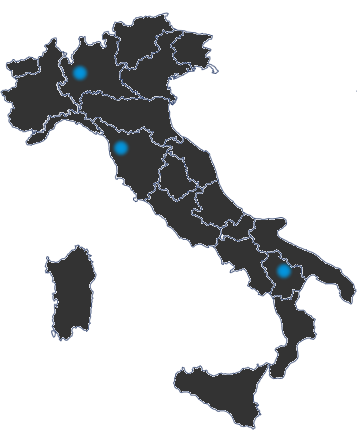
\includegraphics[scale=0.25]{img/italia.png}
%    ~
%  \section{Languages}
%    \textbf{Italian}\includegraphics[scale=0.40]{img/5stars.png}
%    \textbf{English}\includegraphics[scale=0.40]{img/4stars.png}
%\end{aside}
%
%\section{Publications}
%C. Benedetto, E. Mingozzi, C. Vallati\\
%\textbf{A Handoff Algorithm based on Link Quality Prediction for Mass Transit Wireless Mesh Networks}\\
%\emph{Proceedings of the 18th IEEE Symposium on Computers and Communications (ISCC 2013), Split, Croatia, July 7-10, 2013}
%\\
%\section{Other Info}
%For the Italian job market:\\
%\emph{Si autorizza il trattamento delle informazioni contenute nel curriculum in conformità alle disposizioni previste dal d.lgs. 196/2003. Si dichiara altresì di essere consapevole che, in caso di dichiarazioni non veritiere, si è passibili di sanzioni penali ai sensi del DPR 445/00 oltre alla revoca dei benefici eventualmente percepiti.}
%\\
%\begin{flushleft}
%\emph{January 14th, 2014}
%\end{flushleft}
%%\begin{flushright}
%%\emph{Carmine Benedetto}
%\end{flushright}

%%% This piece of code has been commented by Karol Kozioł due to biblatex errors. 
% 
%\printbibsection{article}{article in peer-reviewed journal}
%\begin{refsection}
%  \nocite{*}
%  \printbibliography[sorting=chronological, type=inproceedings, title={international peer-reviewed conferences/proceedings}, notkeyword={france}, heading=subbibliography]
%\end{refsection}
%\begin{refsection}
%  \nocite{*}
%  \printbibliography[sorting=chronological, type=inproceedings, title={local peer-reviewed conferences/proceedings}, keyword={france}, heading=subbibliography]
%\end{refsection}
%\printbibsection{misc}{other publications}
%\printbibsection{report}{research reports}

%\end{document}
